\documentclass[UTF8,zihao=5,a4paper]{ctexart}

\usepackage{amsmath}
\usepackage{geometry}
\geometry{a4paper,scale=0.8}
\usepackage[numbers]{gbt-7714-2015}
% \usepackage[sectionbib]{chapterbib}
\usepackage{minted}
\usepackage{subfigure}
\usepackage{algorithm}
\usepackage{algorithmic}

\newtheorem{Def}{Definition}
\newtheorem{Theo}{Theorem} 


%同济大学机器学习课程报告---ICA理论推导、实现和应用

\title{ICA理论推导、实现和应用}
\author{余海涛 1732985}
\date{}

\begin{document}
    
\begin{titlepage}
    \vspace*{6cm}
    \Huge
    \begin{center}
        \textbf{同济大学机器学习}
        
        \textbf{课程报告}
    \end{center}
    \vspace{3cm}
    \begin{table}[h]
        \Large
        \centering
        \begin{tabular}{|l|c|}
        \hline
        标题 & ICA理论推导、实现和应用\\
        \hline
        姓名 & 余海涛 \\
        \hline
        学号 & 1732985\\        
        \hline
        专业 & 计算机技术\\
        \hline
        班级 & 计算机3班\\
        \hline
        \end{tabular}
    \end{table}
\end{titlepage}

\maketitle

\begin{abstract}
    本篇报告从基础出发对独立成分分析(ICA)理论进行了问题定义和数学推导,给出了ICA问题的数学表达,和非高斯性的理论基础,并基于峭度推导出了快速不动点迭代公式,基于Python实现了FastICA算法,并结合实例展示了ICA的实际应用,通过实验展示了FastICA算法的实际效果,对之前的一些不清晰的案例进行了解释。是对ICA理论的一次学习总结。
\end{abstract}


\section{问题背景}
在统计学中,独立成分分析\cite{icawikipedia,ica,icachinese}(Independent components analysis,缩写:ICA)是一种利用统计原理进行计算的方法。它是一个线性变换。这个变换把数据或信号分离成统计独立的非高斯的信号源的线性组合。独立成分分析是盲信号分离(Blind source separation)的一种特例。

独立成分分析的最重要的假设就是信号源统计独立。这个假设在大多数盲信号分离的情况中符合实际情况。即使当该假设不满足时,仍然可以用独立成分分析来把观察信号统计独立化,从而进一步分析数据的特性。独立成分分析的经典问题是“鸡尾酒会问题”(cocktail party problem)。该问题描述的是给定混合信号,如何分离出鸡尾酒会中同时说话的每个人的独立信号。当有N个信号源时,通常假设观察信号也有N个(例如N个麦克风或者录音机)。该假设意味着混合矩阵是个方阵,即$J = D$,其中$D$是输入数据的维数,$J$是系统模型的维数。对于$J < D$和$J > D$的情况,学术界也分别有不同研究。

鸡尾酒会问题的原始阐述如下。假设你在一个房间里,有三个人在同时讲话,还有三个麦克风,摆放在不同的位置进行录音,麦克风记录下的三个信号可以表示为$x_1(t)$,$x_2(t)$和$x_3(t)$,其中$t$表示时间,$x_1$,$x_2$,$x_3$表示信号幅值,可以认为每一个信号都是三个讲话者发出的信号的加权和,假设三个讲话者的信号用$s_1(t)$,$s_2(t)$和$s_3(t)$表示,则$x_i$和$s_i$的关系可以用线性方程的形式表示为
\begin{equation}
    \left\{
        \begin{aligned}
            x_1(t)=a_{11}s_1(t)+a_{12}s_2(t)+a_{13}s_3(t) \\
            x_2(t)=a_{21}s_1(t)+a_{22}s_2(t)+a_{23}s_3(t) \\
            x_3(t)=a_{31}s_1(t)+a_{32}s_2(t)+a_{33}s_3(t)
        \end{aligned}
    \right.
\end{equation}
式中$a_{ij}(i,j=1,\ldots,3)$是由麦克风与讲话者距离决定的未知数,这里都是未知数,注意这里的模型忽略了录音的时延和其他影响因素,假设三个录音机的采样是同步的,则如何只根据最终的三个录音信号,得到变换的参数和最初的信号,就是独立成分分析要解决的问题。



\section{理论推导}

本节给出ICA理论的具体数学推导,推导的过程主要参考了\cite{icachinese,ica,fastica,icatutorial}。

\subsection{问题定义}
可以使用统计上的“隐变量”模型定义ICA问题,假设观察到$n$个随机变量$x_1,x_2,\ldots,x_n$,而这些变量是由另外$n$个随机变量$s_1,s_2,\ldots,s_n$线性组合得到,可以用矩阵形式表示如下
\begin{equation}
    \mathbf{x}=\mathbf{As}
\end{equation}
其中
\begin{equation}
    \mathbf{x}=\left(
        \begin{aligned}
        x_1\\
        x_2\\
        \vdots\\
        x_n
        \end{aligned}
    \right),
    \mathbf{s}=\left(
        \begin{aligned}
        s_1\\
        s_2\\
        \vdots\\
        s_n
        \end{aligned}
    \right),
    \mathbf{A}=\left(
        \begin{array}{cccc}
        a_{11} & a_{12} & \cdots & a_{1n} \\ 
        a_{21} & a_{22} & \cdots & a_{2n} \\ 
        \vdots & \vdots & \ddots & \vdots \\ 
        a_{n1} & a_{n2} & \cdots & a_{nn}
        \end{array} 
    \right)
\end{equation}

\textbf{假设和约束}:为了确保ICA模型可以被估计,必须做出下面的假设和约束
\begin{enumerate}
    \item 假设独立成分是统计独立的
    \item 独立成分具有非高斯的分布
    \item 未知的混合矩阵是方阵
\end{enumerate}

\textbf{ICA中的不确定性}:在以上定义的ICA模型中,可以发现存在下面一些不确定性
\begin{enumerate}
    \item 无法确定独立成分的方差
    \item 无法确定独立成分的次序
\end{enumerate}

\textbf{变量的中心化}:不失一般性,我们可以假定所有的混合变量与独立成分均具有零均值。这作为下面推导的一个默认假设,如果实际情况不满足零均值假设,可以进行中心化的预处理:
\begin{equation} 
    \mathbf{x}=\mathbf{x'}-E{\mathbf{x'}}
\end{equation}
这样独立成分也同时变为零均值的量,因为:
\begin{equation}
    E{\mathbf{s}}=\mathbf{A}^{-1}E{\mathbf{x}}
\end{equation}

\textbf{不相关性和白化}:不相关性是独立性的一个弱化的形式。如果两个随机变量$y_1$和$y_2$的协方差为零,我们说这两个变量是不相关的:
\begin{equation}
    cov(y_1,y_2)=E\{y_1y_2\}-E\{y_1\}E\{y_2\}=0
\end{equation}
如果随机变量是相互独立的,那么他们就是不相关的,但是不相关并不意味着独立。

白化性(whiteness)是指一个零均值的随机向$y$的各个分量具有相同的单位方差且互相不相关,换句话说$y$的协方差矩阵是单位矩阵:
\begin{equation}
    E\{\textbf{yy}^T\}=\mathbf{\mathit{I}}
\end{equation}
白化意味着我们将观察得到的数据向量$\mathbf{x}$与某个矩阵$\mathbf{V}$相乘后得到的是一个新的白化的向量:
\begin{equation}
    \mathbf{z}=\mathbf{Vx}
\end{equation}
白化变换总是可实现的,一般可以利用协方差矩阵的特征值分解(EVD):
\begin{equation}
    E\{\textbf{xx}^T \}=\textbf{EDE}^T
\end{equation}
式中,$\mathbf{E}$是$E\{\mathbf{xx}^T \}$的特征向量的正交矩阵,$\textbf{D}$是相应的特征向量的对角矩阵,$D=diag\{d_1,d_2,\cdots,d_n\}$。这样,白化过程可以利用下面的白化矩阵来实现:
\begin{equation}
    \mathbf{V}=\mathbf{E}\mathbf{D}^{-1/2}\mathbf{E}^T
\end{equation}
式中,矩阵$\mathbf{D}^{-1/2}=diag\{d_1^{-1/2},d_2^{-1/2},\cdots,d_n^{-1/2}\}$。这样得到的白化矩阵记为$E{\mathbf{xx}^T}^{-1/2}$或$\mathbf{C}^{-1/2}$。在后文的推导过程中,对数据的白化处理也是很重要的一个环节。


\subsection{极大化非高斯性的ICA估计方法}

\textbf{关于非高斯性}:如果两个独立成分$s_1$和$s_2$是高斯分布的,则它们的联合概率密度可以表示为:
\begin{equation}
p(s_1,s_2)
=\frac{1}{2\pi}exp(-\frac{s_1^2+s_2^2}{2})
=\frac{1}{2\pi}exp(-\frac{{\lVert \mathbf{s} \rVert}^2}{2})
\end{equation}
假定混合矩阵是正交的。根据概率密度函数的变换公式(参见附录\ref{apx:1}),根据正交矩阵的特点,$\textbf{A}^{-1}=\textbf{A}^T$成立,可以得到混合变量$x_1$和$x_2$的联合密度函数为:
\begin{equation}
p(x_1,x_2)
=\frac{1}{2\pi}exp(-\frac{{\lVert \mathbf{A}^T\mathbf{x} \rVert}^2}{2})|\text{det}\,\mathbf{A}^T|    
\end{equation}
由$\mathbf{A}$的正交性可知${\lVert \mathbf{A}^T\mathbf{x} \rVert}^2={\lVert \mathbf{x} \rVert}^2$和$|\text{det}\,\mathbf{A}|=1$成立。另外如果$\textbf{A}$是正交的,其转置$\textbf{A}^T$也同样是正交的。因此我们有:
\begin{equation}
p(x_1,x_2)
=\frac{1}{2\pi}exp(-\frac{{\lVert \mathbf{x} \rVert}^2}{2})
\end{equation}
这里可以看出混合变量的概率密度函数和原始的概率密度函数都是二维高斯分布,我们没有任何办法得到混合矩阵的信息。

\textbf{极大化非高斯性的原理}:中心极限定理是概率论中的一个经典结论,该定理告诉我们,独立的随机变量之和的分布趋向于高斯分布。或者不那么严格的讲,可以认为两个独立随机变量之和形成的分布比两个原始的随机变量中的任意一个更接近于高斯分布。

现在为了估计出ICA数据模型中的一个独立成分,我们先假定所有独立成分具有相同的分布,可以考虑对$x_i$进行某种线性组合,有:
\begin{equation}
    y=\mathbf{b}^T\mathbf{x}=\mathbf{q}^T\mathbf{s}=\sum_{i}q_is_i
\end{equation}
如果$\mathbf{b}$是$\mathbf{A}^{-1}$中的一行,那么该线性组合$\mathbf{b}^T\mathbf{A}$就等于其中一个独立成分,而对应的向量$\mathbf{q}$只有一个元素为1,其他的元素均为0.

问题在于:我们如何使用中心极限定理确定$\mathbf{b}$,是的它刚好等于$\mathbf{A}$的逆矩阵中的一行?实际上,我们无法准确地得到这样地$\mathbf{b}$,因为没有关于矩阵$\mathbf{A}$的先验知识,但是可以找到具有较好近似程度的一个估计。

我们可以通过改变$\mathbf{q}$中的系数来观察$y=\mathbf{q}^T\mathbf{s}$的分布如何变化。这里的基本思想是,既然两个独立随机变量之和分布的高斯性都比原始变量的更强,那么$y=\mathbf{q}^T\mathbf{s}$应该比任意一个$s_i$的高斯性更强,除非y刚好就是$s_i$中的一个,只有在该情况下y的高斯性才最弱(注意,该结论只有在假定所有$s_i$具有相同分布的情况下才严格成立)。这是显然$\mathbf{q}$中只有一个元素$q_i$为非零值。

实际情况下我们并不知道$\mathbf{q}$的值,但也无须知道,因为根据定义$\mathbf{b}^T\mathbf{x}=\mathbf{q}^T\mathbf{s}$,可以只让$\mathbf{b}$变化并观察$\mathbf{b}^T\mathbf{x}$的分布变化情况。因此可以直接把变量$\mathbf{b}$用于极大化$\mathbf{b}^T\mathbf{x}$的非高斯性,这样的向量对应于$\mathbf{q}=\mathbf{A}^T\mathbf{b}$只有一个非零元素的情形,从而意味着$ y=\mathbf{b}^T\mathbf{x}=\mathbf{q}^T\mathbf{s}$正好等同于独立成分中的一个。也就是说通过极大化$\mathbf{b}^T\mathbf{x}$的非高斯性,就能给出其中一个独立成分。






\section{算法实现}

上一节给出了计算一个分量的基于峭度的快速不动点迭代公式,基于该公式可以得到ICA的有效算法,常被称为FastICA算法。但实际上,ICA算法推导可以使用不同的非高斯性度量或者使用不同的推导准则,可以得到多种ICA算法,其中最常用的是基于负熵的快速不动点算法,也是更为高效的FastICA算法,表\ref{fast_ica_alg}给出了使用对称正交化方法的可以估计多个独立成分的FastICA算法,参考文献\cite{ica}:

\begin{table}[h]
    \centering 
    \begin{tabular}{p{0.8\columnwidth}}
        \hline 
        1. 对数据进行中心化使其均值为0\\
        2. 然后对数据进行白化得到$z$\\
        3. 选择要估计的独立成分个数$m$\\
        4. 初始化所有的$\mathbf{w}_i,i=1,2,\cdots,m$,其中每个$\mathbf{w}_i$都具有单位范数。用下面第6步的方法对矩阵$\mathbf{W}$进行正交化\\
        5. 对每一个$i=1,2,\cdots,m$,更新$\mathbf{w}_i$:$\mathbf{w}_i\leftarrow E\{ \mathbf{z} g(\mathbf{w}_i^T\mathbf{z}) \}-E\{ g'(\mathbf{w}_i^T\mathbf{z}) \}\mathbf{w}_i$,其中g的形式可以取$g_1(y)=tanh(a_1y)$或$g_2(y)=y\,exp(-y^2/2)$或$g_3(y)=y^3$\\
        6. 对矩阵$\mathbf{W}=(\mathbf{w_1},\cdots,\mathbf{w_n})^T$进行正交化:$\mathbf{W}\leftarrow(\mathbf{WW}^T)^(-1/2)\mathbf{W}$\\
        7. 如果没有收敛,则返回步骤5\\
        \hline 
    \end{tabular} 
    \caption{估计多个独立成分的FastICA算法,使用对称正交化方法。实际应用中,期望用样本的平均值来估计}
    \label{fast_ica_alg}
\end{table}

%\begin{table}[h]
%    \centering
%    \begin{tabular}{l}
%        \hline 
%        1. 对数据进行中心化使其均值为0\\
%        2. 然后对数据进行白化得到$z$\\
%        3. 选择要估计的独立成分个数$m$。置$p\leftarrow 1$\\
%        4. 选择具有单数范数的初始化向量$w_p$(可随机选取)\\
%        5. 更新$w_p$:$w_p\leftarrow E\{zg(w_P^T z)\}-E\{g'(w_p^T z)w_p\}$,其中g的定义可以取\\
%        6. 进行下面的正交化
%        $\mathbf{w}_p\leftarrow \mathbf{w}_p-\sum_{j=1}^{p-1}(\mathbf{w}_p^T \mathbf{w}_j)\mathbf{w}_j$ \\
%        7. 标准化$w_p$,即 $\mathbf{w}_p\leftarrow \mathbf{w}_p/\lVert \mathbf{w}_p \rVert$\\
%        8. 如果$\mathbf{w}_p$尚未收敛,返回步骤5\\
%        9. 置$p\leftarrow p+1$。如果$p\leq m$,返回步骤4\\
%        \hline 
%    \end{tabular} 
%    \caption{估计多个独立成分的FastICA算法,使用渐进(串行)正交化方法。实际应用中,期望用样本的平均值来估计}
%    \label{fast_ica_alg}
%\end{table}

本文基于Python平台具体实现了FastICA的算法,核心代码及注释如下:

\begin{minted}{python}
import math
import random
import matplotlib.pyplot as plt
from numpy import *

n_components = 2

def f1(x, period = 4):
    return 0.5*(x- math.floor(x/ period )* period )

def create_data ():
    n = 500 # data number
    T = [0.1*xi for xi in range (0, n)] # data time
    S = array([[sin(xi) for xi in T], [f1(xi) for xi in T]],float32) # source
    A = array([[0.8, 0.2], [-0.3, -0.7]], float32) # mix matrix
    return T, S, dot(A, S)

def whiten (X):
    # 零均值
    X_mean = X.mean(axis =-1)
    X -= X_mean [:, newaxis ]
    # 白化
    A = dot(X, X.transpose ())
    D , E = linalg.eig(A)
    D2 = linalg.inv( array ([[D[0], 0.0], [0.0, D[1]]], float32 ))
    D2[0,0] = sqrt(D2[0,0]); D2[1,1] = sqrt (D2[1,1])
    V = dot(D2 , E.transpose ())
    return dot(V, X), V

def _logcosh (x, fun_args =None , alpha = 1):
    gx = tanh(alpha * x, x); g_x = gx ** 2
    g_x -= 1.; g_x *= - alpha
    return gx , g_x.mean( axis =-1)

def do_decorrelation (W):
    s, u = linalg.eigh(dot(W, W.T))
    return dot(dot(u * (1./sqrt(s)), u.T), W)

def do_fastica (X):
    n, m = X. shape ; p = float(m); g = _logcosh
    X *= sqrt(X.shape[1])
    # create w
    W = ones((n,n), float32 )
    for i in range(n):
        for j in range(i):
            W[i,j] = random.random()
    # compute W
    maxIter = 200
    for ii in range ( maxIter ):
        gwtx , g_wtx = g(dot(W, X))
        W1 = do_decorrelation ( dot(gwtx , X.T) / p - g_wtx [:,newaxis ] * W)
        lim = max ( abs (abs ( diag (dot (W1 , W.T))) - 1) )
        W = W1
        if lim < 0.0001:
            break
    return W

def main():
    T, S, D = create_data()
    Dwhiten , K = whiten (D)
    W = do_fastica( Dwhiten )
    Sr = dot( dot(W, K), D)
    for i,M in enumerate((D,S,Sr),1):
        plt.subplot(3,1,i)
        plt.plot(T, [M[0,i] for i in range (S.shape[1])], marker ="*")
        plt.plot(T, [M[1,i] for i in range (S.shape[1])], marker ="o")
    plt.show()
    print(W)
\end{minted}


\section{实际应用}
如前文所述,ICA算法的一个实际应用是盲信号分离。本节先给出一个分离三个合成的周期信号的例子\cite{example} 。结果如图\ref{fig:result1}和图\ref{fig:result2}所示,无论在有无高斯噪声的情况下,ICA均重构出了原始信号,说明ICA方法可以有效的解决盲信号分离的问题。

\begin{figure}[h]
    \centering
    \includegraphics[width=0.9\linewidth]{figs/result1}
    \caption{无高斯噪声情况下的ICA分离结果}
    \label{fig:result1}
\end{figure}


\begin{figure}[h]
    \centering
    \includegraphics[width=0.9\linewidth]{figs/result2}
    \caption{有高斯噪声情况下的ICA分离结果}
    \label{fig:result2}
\end{figure}

在实际中,ICA也被用于图像处理、语言识别、通信、生物医学信号处理、脑功能成像研究、故障诊断、特征提取、金融时间序列分析和数据挖掘等多个领域。如图\ref{fig:face}所示是对人脸数据进行降维得到的数据,对比经典的PCA方法,可以看到ICA方法也可以起到降低数据维度的作用,而且可以反映人脸的不同特征。

\begin{figure}[h]
    \centering
    \subfigure[原始人脸]{
        \label{fig:face0}
        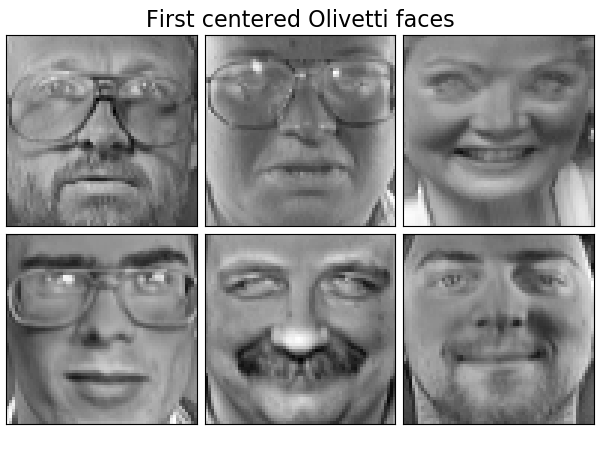
\includegraphics[width=1.5in]{figs/face0.png}
    }
    \hspace{0.2in}
    \subfigure[PCA降维]{
        \label{fig:face1}
        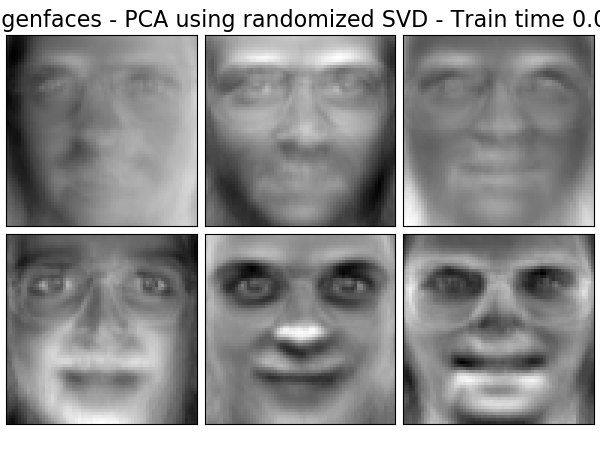
\includegraphics[width=1.5in]{figs/face1.png}
    }
    \hspace{0.2in}
    \subfigure[ICA降维]{
        \label{fig:face2}
        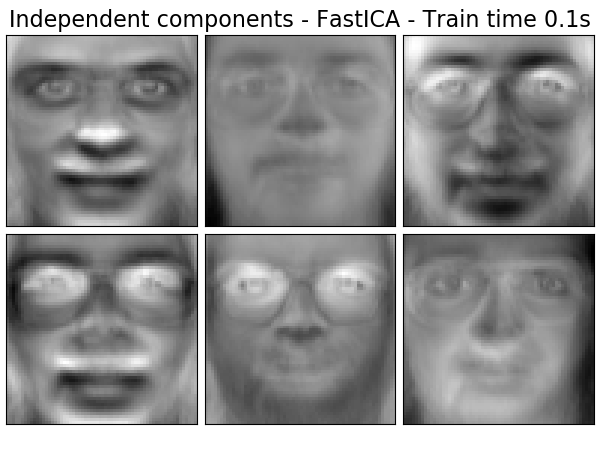
\includegraphics[width=1.5in]{figs/face2.png}
    }
    \caption{人脸图像降维示例}
    \label{fig:face}
\end{figure}


本节最后给出一个分离混合音频信号的例子程序。通过实际的体验,可以发现ICA可以很好的分离线性混合后的音频,并且恢复原始音频,说明ICA可以有效解决理想情况下的鸡尾酒会问题,但是值的注意的是,在现实实验中由于存在录音的误差和信号采样时钟的延迟问题,对于现实场景问题下的鸡尾酒会问题,ICA方法仍然存在很多不适宜的地方。

\section{总结}
本文分析了ICA理论的问题定义和数学原理,给出了ICA问题的数学表达,和非高斯性的理论基础,并基于峭度推导出了快速不动点迭代公式,实现了FastICA算法,并且实际分析了ICA算法的效果,从最终实验的结果可以看到,FastICA算法很好的达到了分离原始信号的目的。本文也展示了ICA在多个领域的应用。通过本文的写作,本人对ICA算法有了清晰的认识,对机器学习算法里的数理逻辑有了进一步的认识,可以很好地用于以后的研究中。

% \gbtbibstyle{numerical}
% \bibliographystyle{gbt-7714-2015-numerical}
\bibliography{ref}



\newpage
{\noindent\LARGE{\textbf{附录}}}
\begin{appendix}
\section{概率密度函数的变换}\label{apx:1}
假定$x$和$y$都是n维随机向量,通过下述向量映射相联系:
\[
    \mathbf{y}=\mathbf{g}(\mathbf{x})
\]
此映射的逆变换存在且唯一,为:
\[
    \mathbf{x}=\mathbf{g}^{-1}(\mathbf{y})
\]
可以利用$\mathbf{x}$的概率密度分布函数$p_x(\mathbf{x})$得到$\mathbf{y}$的密度$p_y(\mathbf{y})$:
\[
    p_y(\mathbf{y})=
    \frac{1}{| det\,\mathit{J}\mathbf{g}(\mathbf{g}^{-1}(\mathbf{y}) ) |}
    p_x(\mathbf{g}^{-1}(\mathbf{y}))
\]
式中,$\mathit{J}\mathbf{g}$是雅可比矩阵:
\[
    \mathit{J}\mathbf{g}(\mathbf{x})=\left[
    \begin{array}{cccc}
    \frac{\partial g_1(\mathbf{x})}{\partial x_1}&  \frac{\partial g_2(\mathbf{x})}{\partial x_1}&  \cdots&  \frac{\partial g_n(\mathbf{x})}{\partial x_1}\\ 
    \frac{\partial g_1(\mathbf{x})}{\partial x_2}&  \frac{\partial g_2(\mathbf{x})}{\partial x_2}&  \cdots&  \frac{\partial g_n(\mathbf{x})}{\partial x_2}\\ 
    \vdots&  \vdots&  \ddots&  \vdots\\ 
    \frac{\partial g_1(\mathbf{x})}{\partial x_n}&  \frac{\partial g_2(\mathbf{x})}{\partial x_n}&  \cdots&  \frac{\partial g_n(\mathbf{x})}{\partial x_n}\\ 
    \end{array} 
    \right]
\]

\section{不动点迭代}\label{apx:2}
\begin{Def}
    \textbf{不动点}:对于给定的函数$\varphi$,如果一个数$x$满足$\varphi(x)=x$,则这个数是一个不动点
\end{Def}

不动点迭代算法如算法\ref{alg:apxB}所示,
\begin{algorithm}
    \caption{不动点迭代}  
    \label{alg:apxB}
    \begin{algorithmic}  
        \STATE {将$f(x)=1$转化为$x=g(x)$的形式}
        \STATE {初始化$x=x_0$}   
        \REPEAT
        \STATE $x_{i+1}=g(x_i)$
        \UNTIL {满足收敛条件$C_1$和$C_2$} 
    \end{algorithmic}  
\end{algorithm}

迭代过程的收敛性定理如定理\ref{theo:apxB}所示,

\begin{Theo}
    \label{theo:apxB}
    设迭代函数$\varphi(x)$在$[a,b]$上连续,且满足
    
    $C_1$\ 当$x\in [a,b]$时,$a\leq\varphi(x)\leq b$;
    
    $C_2$\ 存在以正数$L$,满足$0<L<1$,且$\forall x\in [a,b]$,有$|\varphi '|\leq L$
    
    则有,
    
    1. 方程$x=\varphi(x)$在$[a,b]$内有唯一解$x^*$
    
    2. 对于任意初值$x_0\in [a,b]$,迭代法均收敛于$x^*$
    
    3. $|x_k-x^*|\leq \frac{L}{1-L}| x_k-x_{k-1} |$
    
    4. $|x_k-x^*|\leq \frac{L^k}{1-L}| x_1-x_0 |$
\end{Theo}

\end{appendix}

\end{document}    








